\section{Desenvolvimento Experimental}
\subsection{Materiais e Métodos}
<<<<<<< HEAD
Foi utilizado para o experimento o equipamento PASCO Modelo OS-9171 cosntituido por: 
=======
Foi utilizado para o experimento o equipamento PASCO Modelo OS-8501 cosntituido por: 
>>>>>>> f8d5dbf13b81f1364abbea5dea07f67d646da400
\begin{itemize}
	\item Espelho fixo (M1);
	\item Espelho móvel (M2);
	\item Separador de feixes (\it{beam-splitter});
	\item Micrômetro;
	\item Câmara de vácuo.
\end{itemize}
Sendo utilizado também:
\begin{itemize}
	\item Lasers (um com comprimento de onda conhecido e outro a determinar);
	\item Lente divergente.
\end{itemize}

<<<<<<< HEAD
    O primeiro passo é alinhar o laser de comprimento de onda conhecido com o espelho móvel da base do interferômetro - é importante que o raio refletido seja desviado poucos milímetros do orifício do laser, evitando reflexões em seu interior. Após, insere-se a lente divergente entre o laser e o \it{beam-splitter}, posicionado a 45º de forma que o feixe seja parcialmente refletido para o espelho fixo, como consequência deve-se ver um padrão de franjas claras/escuras na superfície de projeção. Caso sejam formados dois padrões de franjas, deve-se ajustar o espelho fixo para que ambas se sobreponham. 
    Recomenda-se demarcar na superfície de projeção os limites de uma das franjas para facilitar a contagem durante o experimento, outra sugestão é a de se usar uma câmera fotográfica com filmagem em câmera lenta durante a contagem. 
    
\subsection{Dados Obtidos Experimentalmente}
Após a realização do experimento duas vezes, foram obtidos diversos tempos de subida e descida, utilizando os mesmos, foram calculadas as velocidades de subida e descida e também o raio de cada gota, como é possível ver na tabela \ref{tab:Vel}
\begin{table}[!htb]
\centering
\begin{tabular}{l|ll|ll|ll|}

Gota & $Vel_f \times 10^{-5} (m/s)$ & $Delta Vel_f$ & $Vel_r \times 10^{-5} (m/s)$ & $Delta Vel_r$ & $a \times 10^{-7} (m)$ & $Delta a$ \\
\rowcolor[HTML]{C0C0C0} 
1    & 4,31                         & 0,3           & 2,03                         & 0,05          & 4,69                   & 0,03      \\ 
2    & 5,58                         & 0,64          & 1,9                          & 0,01          & 5,21                   & 0,16      \\
\rowcolor[HTML]{C0C0C0} 
3    & 3,11                         & 0,02          & 1,64                         & 0,06          & 4,46                   & 0,04      \\
4    & 0,85                         & 0,63          & 0,6                          & 0,33          & 3,68                   & 0,24      \\
\rowcolor[HTML]{C0C0C0} 
5    & 1,11                         & 0,56          & 0,91                         & 0,25          & 3,09                   & 0,4       \\
6    & 2,22                         & 0,26          & 1,5                          & 0,09          & 3,82                   & 0,21      \\
\rowcolor[HTML]{C0C0C0} 
7    & 0,83                         & 0,63          & 0,53                         & 0,35          & 3,98                   & 0,17      \\
8    & 1,68                         & 0,4           & 0,87                         & 0,26          & 4,5                    & 0,03      \\
\rowcolor[HTML]{C0C0C0} 
9   & 3,5                          & 0,08          & 1,89                         & 0,01          & 4,41                   & 0,05      \\
10   & 4,53                         & 0,36          & 1,93                         & 0,02          & 4,87                   & 0,07      \\ \hline
\end{tabular}
\caption{Valores calculados para as velocidades de descida($V_f$), velocidade de subida($V_r$) e o raio de cada gota($a$), assim como o desvio padrão associado a cada medida.}
\label{tab:Vel}
\end{table}

Com os valores obtidos e  utilizando a equação \ref{eq:14} é possível encontrar o valor de carga que cada gota possui, explicito na tabela \ref{tab:Car}.
\begin{table}[!htb]
\centering
\begin{tabular}{l|ll|}
Gota & $Carga \times 10^{-19} (C)$ & $\Delta Carga$ \\
\rowcolor[HTML]{C0C0C0}
1    & 2,22                        & 0,17           \\ 
2    & 2,99                        & 0,38           \\
\rowcolor[HTML]{C0C0C0} 
3    & 1,41                        & 0,05           \\
4    & 0,22                        & 0,37           \\
\rowcolor[HTML]{C0C0C0} 
5    & 0,35                        & 0,33           \\
6    & 0,93                        & 0,18           \\
\rowcolor[HTML]{C0C0C0} 
7    & 0,2                         & 0,37           \\
8    & 0,55                        & 0,28           \\
\rowcolor[HTML]{C0C0C0} 
9   & 1,7                         & 0,03           \\
10   & 2,32                        & 0,2            \\ \hline
\end{tabular}
\caption{Valores da carga associada a cada gota, assim como o seu respectivo desvio padrão.}
\label{tab:Car}
\end{table}

=======
    O primeiro passo é alinhar o laser de comprimento de onda conhecido com o espelho móvel da base do interferômetro - é importante que o raio refletido seja desviado poucos milímetros do orifício do laser, evitando reflexões em seu interior. Após, insere-se a lente divergente entre o laser e o {\it beam-splitter}, posicionado a 45º de forma que o feixe seja parcialmente refletido para o espelho fixo, como consequência deve-se ver um padrão de franjas claras/escuras na superfície de projeção. Caso sejam formados dois padrões de franjas, deve-se ajustar o espelho fixo para que ambas se sobreponham. 
>>>>>>> f8d5dbf13b81f1364abbea5dea07f67d646da400

    Recomenda-se demarcar na superfície de projeção os limites de uma das franjas para facilitar a contagem durante o experimento, outra sugestão é a de se usar uma câmera fotográfica com filmagem em câmera lenta durante a contagem. 
    
Então é realizado a calibração do interferômetro utilizando o laser conhecido, inicialmente é posto a contagem do micrômetro no zero e então feito um deslocamento no espelho móvel utilizando a haste do micrômetro em 20 unidades, e contando quantas franjas são deslocadas é possível calibrar o interferômetro para que o comprimento de onda de qualquer laser possa ser encontrado.

O próximo estágio realizado é para se aferir o índice de refração do ar, é montado o equipamento com o laser de HeNe e antes do espelho fixo é posto uma câmara onde será feito vácuo, então o equipamento é alinhado novamento e variando a pressão na câmara de 10 em 10 mmMg é contado a variação das franjas. 	 
\subsection{Interpretação dos Resultados}
Após a realização da primeira parte do experimento, é encontrado que  cada variação do micrômetro equivale na verdade a $20,2 \times 10^{-6} m$. Substituindo o laser conhecido por um qualquer e utilizando a equação (\ref{eq:lbd}), é possivel encontrar o comprimento de onda do laser.

Para a segunda parte do experimento, foram repetidas as aferições para que o erro fosse reduzido, então com os dados de $\Delta P$ e $\Delta M$ e utilizando a equação (\ref{eq:ni}) são obtidos valores para a confecção do gráfico de $\eta \times \Delta P$ encontrado na figura (\ref{im:aa}).

 \begin{figure}[!h]
 	\centering
 		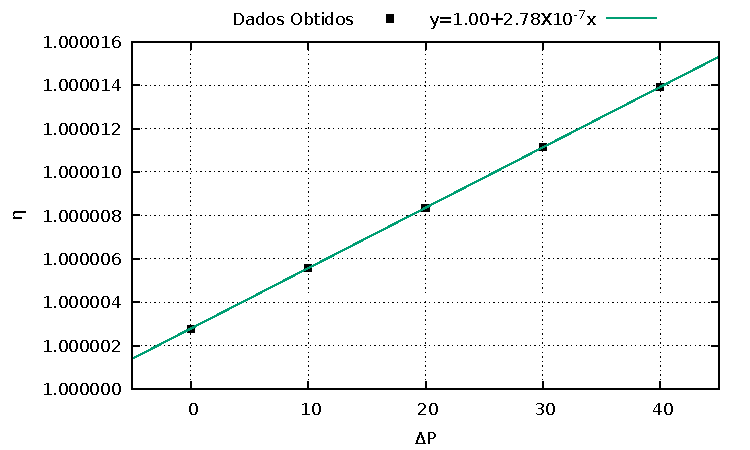
\includegraphics[scale= 1]{grafico/ar.pdf}
 	\caption{Interferômetro de Michelson}
 	\label{im:aa}
 \end{figure}

Assim 
\begin{equation*}
\alpha = \frac{\Delta m\lambda}{2d\Delta P}
\end{equation*}
\begin{equation*}
\alpha = 2.78\times 10^{-7}
\end{equation*}

Calculando o valor do coeficiente angular da reta é possivel encontrar o valor do índice de refração do ar, $\eta_{ar}$, aplicando o valor encontrado na equação (\ref{eq:ni}) e para este experimento foi encontrado $\eta_{exp} = 1.00002052$.

Comparando o valor obtido com o teórico que vale $\eta_{ar} = 1.000293$ é encontrado um desvio percentual de $D\% = 0,0272\%$.
